% \documentclass[a4paper, 12pt, usenames]{report}

% \usepackage[spanish]{babel}
% \usepackage[utf8]{inputenc}
% \usepackage{graphicx}
% \usepackage{caption}
% \usepackage{subcaption}
% %\usepackage{subfigure}
% \usepackage{wrapfig}
% \usepackage{bbding} %Fuentes con iconos lindos

% \usepackage[rflt]{floatflt} %Para meter figuras flotantes entre el texto
% \usepackage[font=footnotesize,labelfont=bf]{caption}
% \usepackage[dvipsnames]{xcolor}
% \usepackage{bclogo} %Iconos bonitos hechos con tikz
% \usepackage{parskip}
% \usepackage{fixmath}

% \usepackage{flushend}

% \usepackage{amsmath}


% \newcommand{\defin}[1]{\bigskip{\large  \color{Orange} \PencilRightDown{} \bf {#1}} }
% \newcommand{\ejerc}[1]{\bigskip{\color{OliveGreen} \FourClowerSolid{} {\bf Ejercitemos nuestra comprensión:}}

%   \vspace*{-0.5\baselineskip}
%   \noindent
%   \rule{17cm}{.5pt}
% #1

% \vspace*{-0.5\baselineskip}
% \noindent
% \rule{17cm}{.5pt}
% \vspace*{-0.5\baselineskip}
% }

% \newcommand{\info}[1]{
% \begin{itemize}
% \item[\bcinfo] {\footnotesize {#1}}
% \end{itemize}
% }

% \topmargin=-2.5cm
% \oddsidemargin=-0.5cm
% \textheight=25cm
% \textwidth=17cm


% \begin{document}



\defin{Posición}

Dar la posición de un cuerpo puntual significa ubicar el punto unívocamente respecto del sistema de coordenadas. Observemos dos ejemplos, en el espacio y en el plano.


\begin{figure}[H]
\centering
\begin{minipage}{.45\textwidth}
\center
  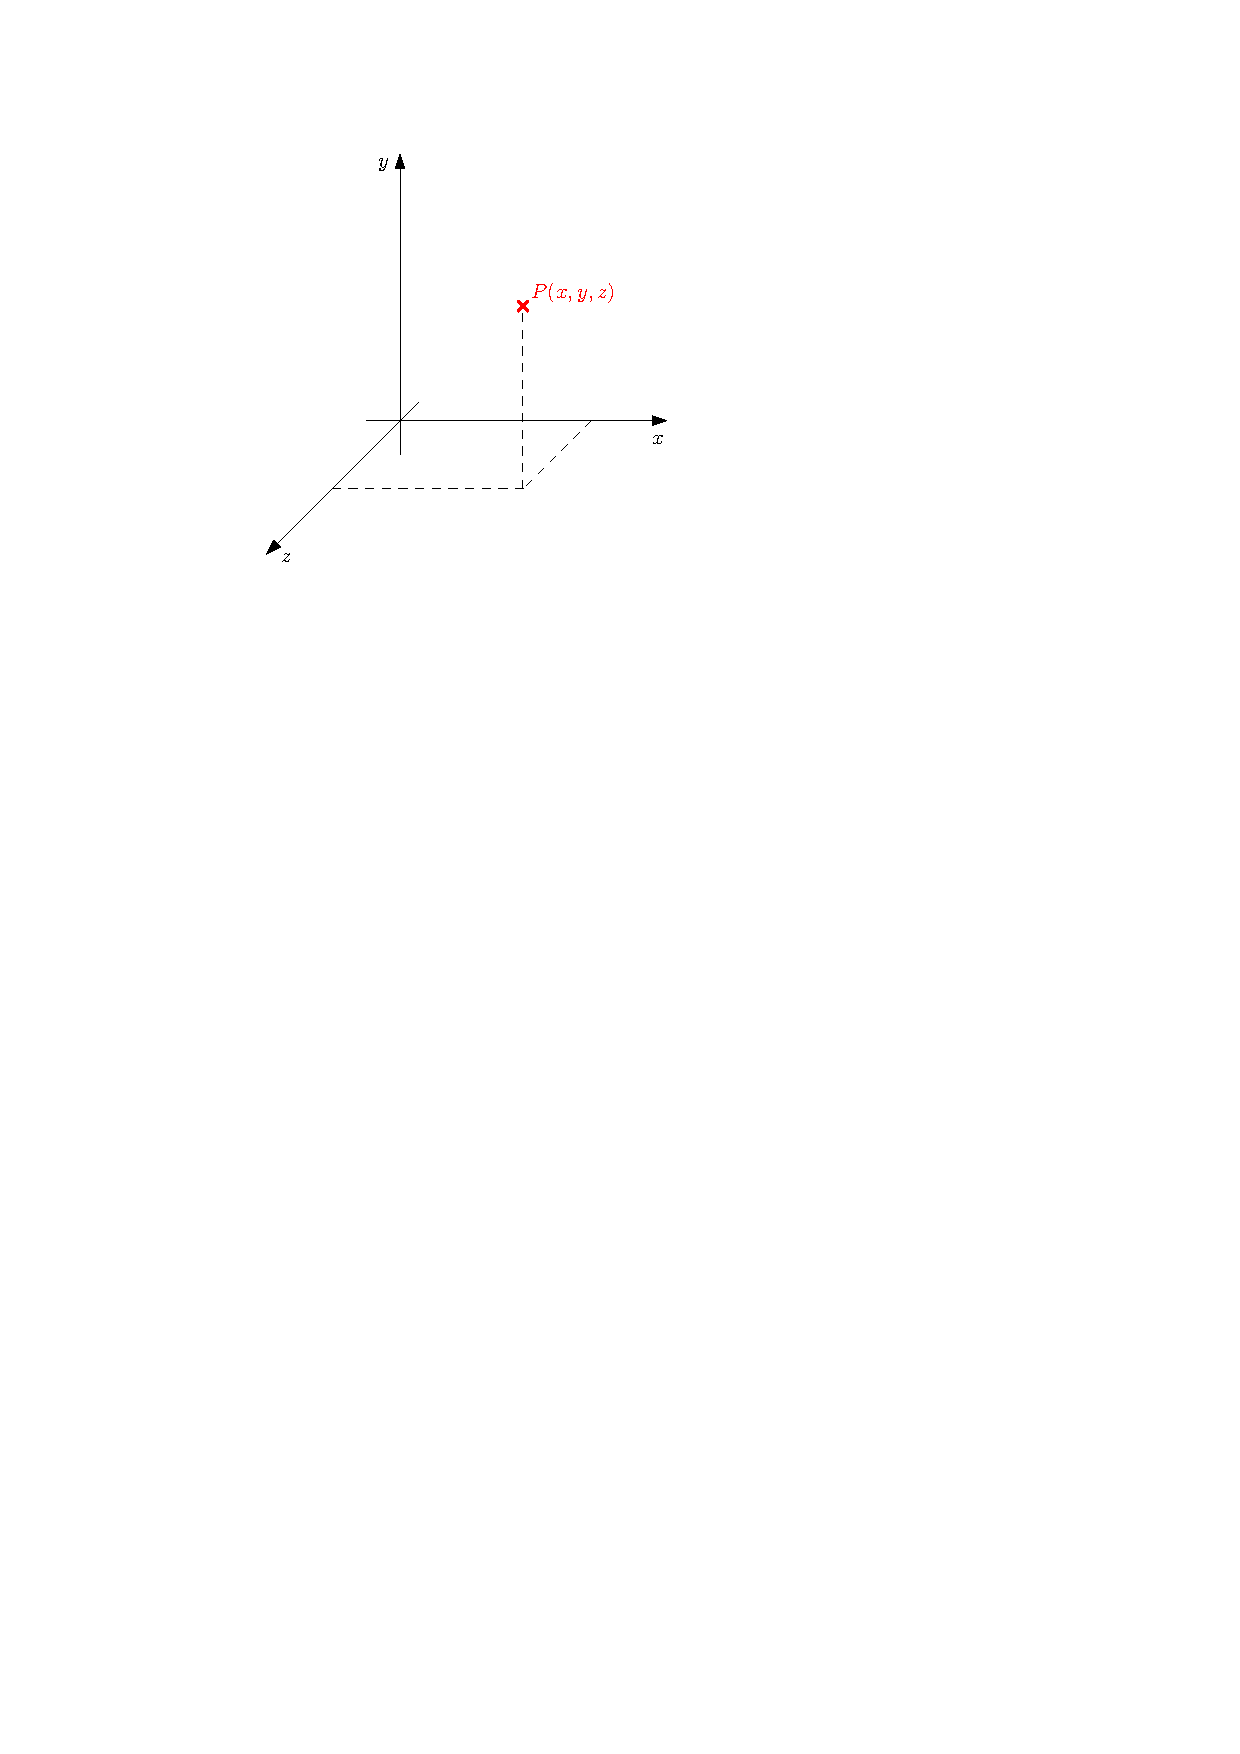
\includegraphics[width=.9\textwidth]{img/3d.pdf}
  \caption{Posición en el espacio.}
\end{minipage}%
\hfill
\begin{minipage}{.45\textwidth}
\center
  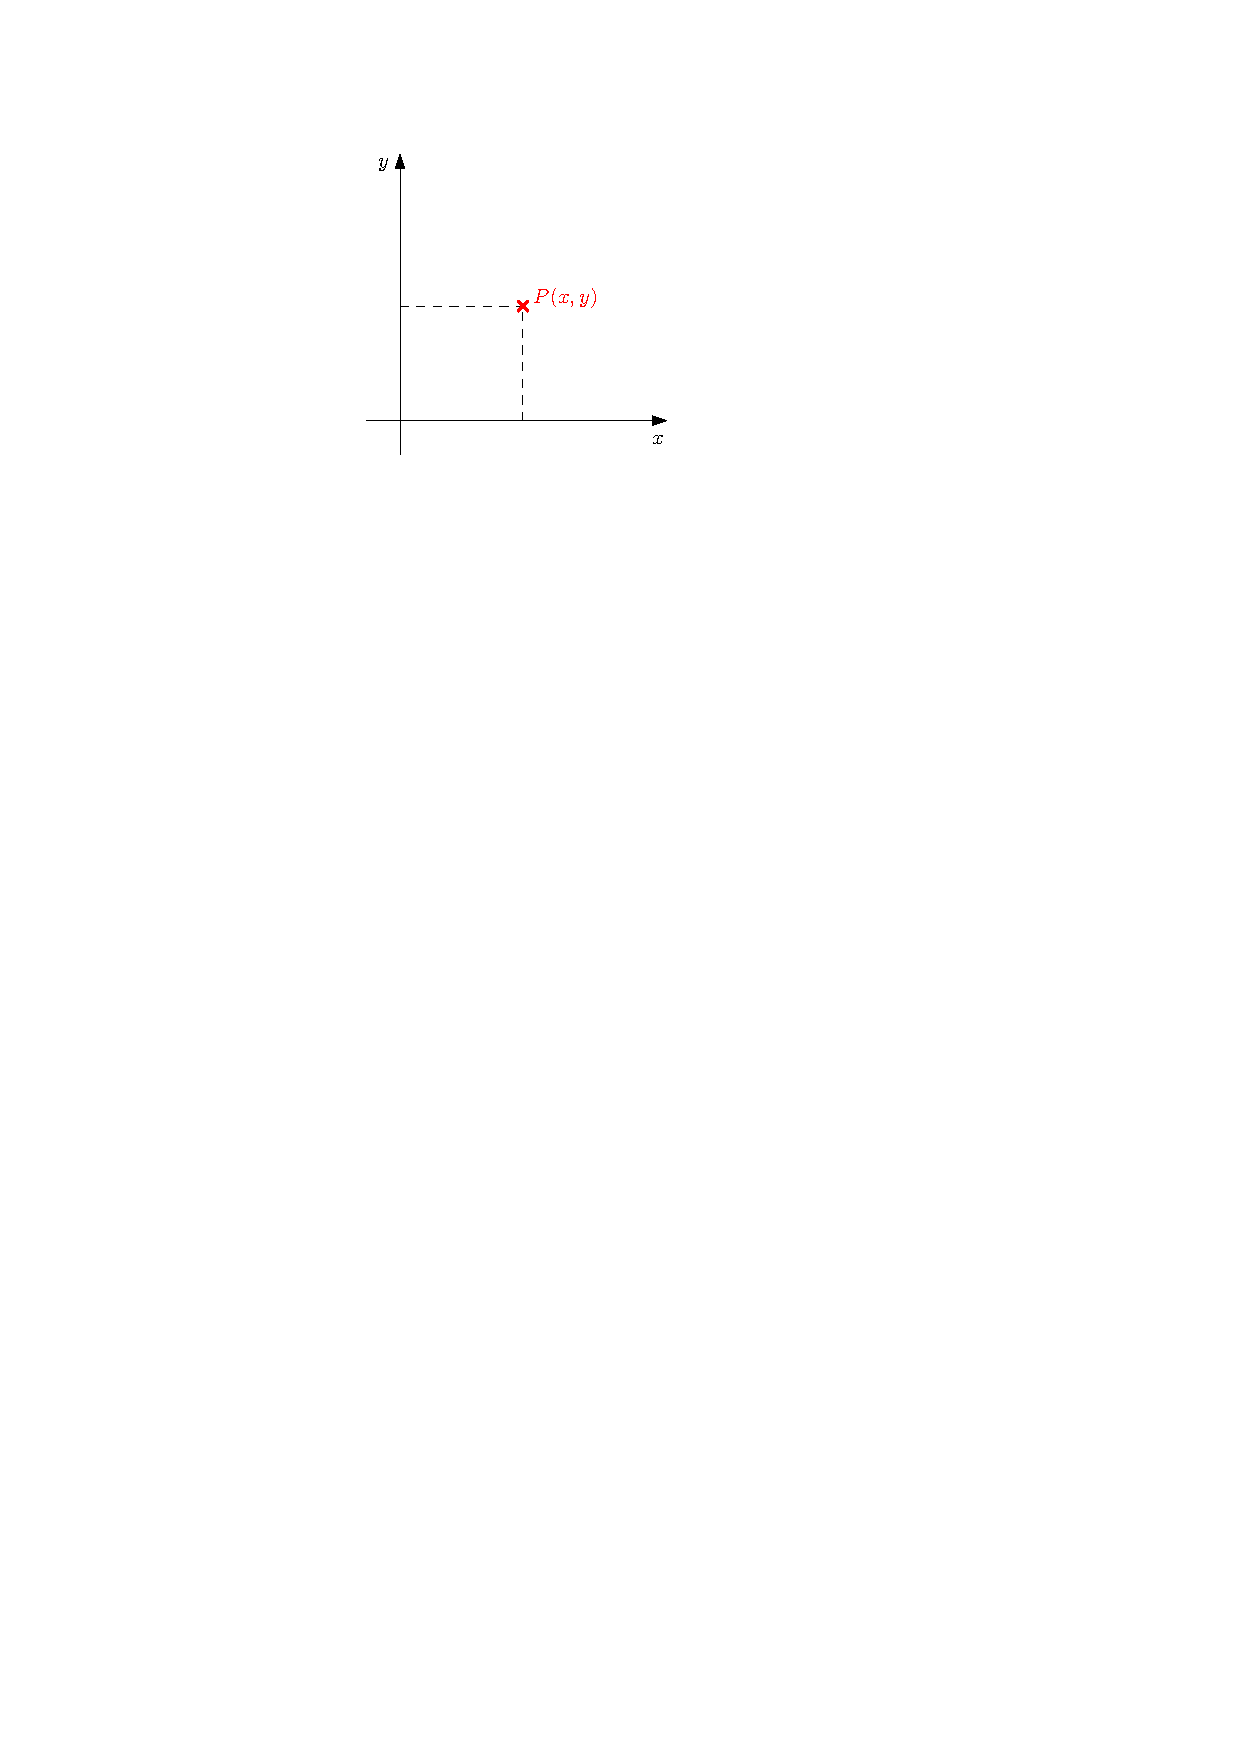
\includegraphics[width=.9\textwidth]{img/2d.pdf}
  \caption{Posición en el plano.}
\end{minipage}
\end{figure}


En los movimientos rectilíneos, para dar la posición de una partícula, sólo necesitamos una magnitud  que represente la distancia entre un punto fijo, el origen de coordenadas, y la ubicación de la partícula. Esta magnitud queda determinada por un número y su unidad. Este número  puede ser  positivo o negativo, según la partícula se encuentre a la derecha o a la izquierda del origen de coordenadas.

\begin{figure}[H]
\center
 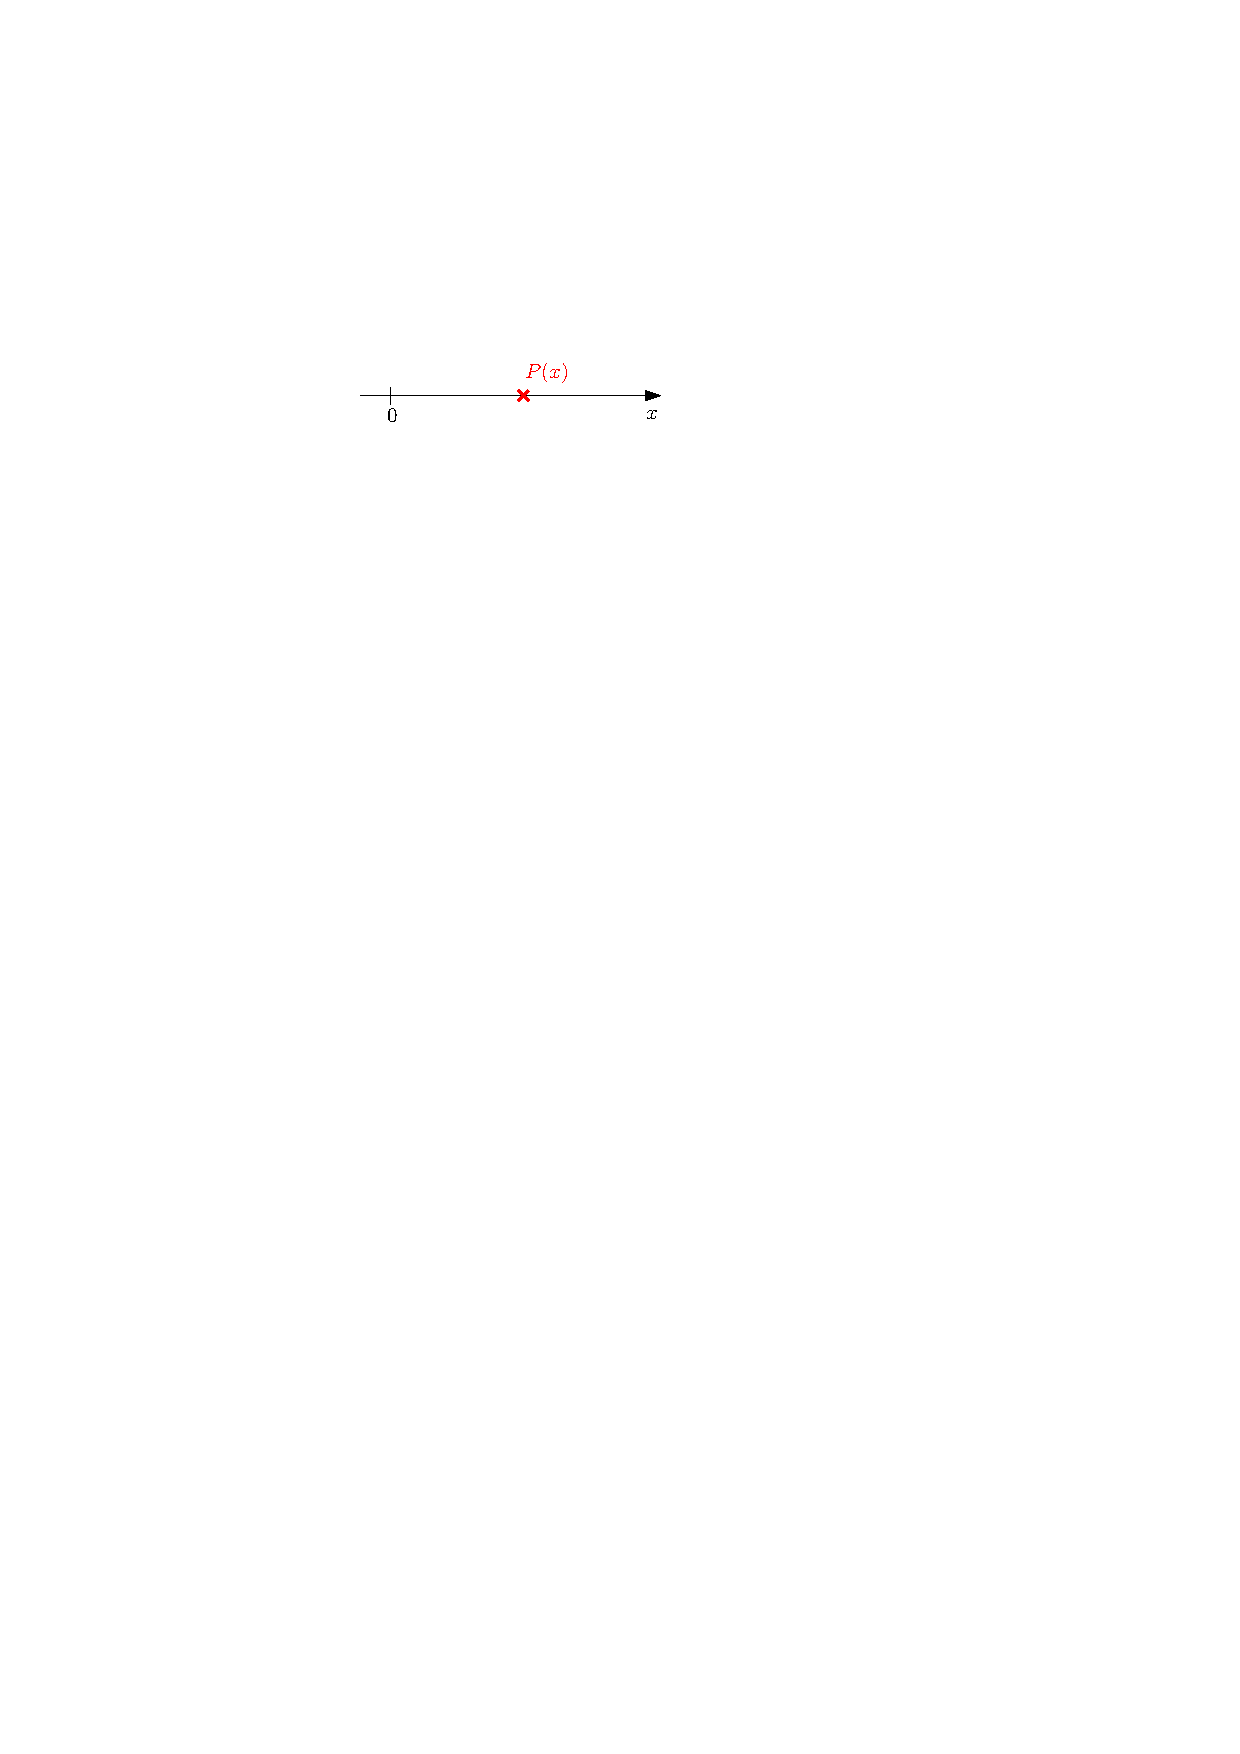
\includegraphics[width=.4\textwidth]{img/1d.pdf}
  \caption{Posición en una dimensión.}
\end{figure}


\defin{Distancia recorrida}

La distancia recorrida se refiere a la longitud de la trayectoria que recorre la partícula en un determinado intervalo de tiempo durante su movimiento.

Es una {\bf magnitud escalar}.



\defin{Desplazamiento}

Cuando una partícula se mueve desde la posición $\mathbold{P_0}$ hasta la posición $\mathbold{P}$, su desplazamiento esta dado por $\mathbold{\bar{d}}$, como observamos en la figura:


\begin{figure}[h!]
\centering
 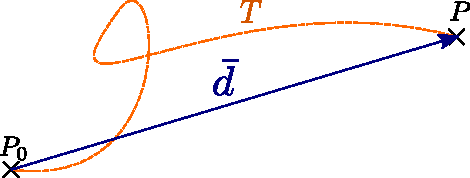
\includegraphics[width=.4\textwidth]{img/trayectoria_distancia.pdf}
  \caption{Desplazamiento de una partícula y la trayectoria de su movimiento.}
\end{figure}


Vemos, entonces, que el desplazamiento es un {\bf vector} con origen en la posición inicial de la partícula {$\mathbold{P_0}$} y extremo en la posición final de la misma {$\mathbold{P}$}. Es decir que \underline{solo} depende de la posición inicial y final de dicha partícula. 

El desplazamiento es una {\bf magnitud vectorial}.


En particular, en un movimiento rectilíneo, el desplazamiento se representa de la siguiente manera:


\begin{figure}[h!]
\centering
 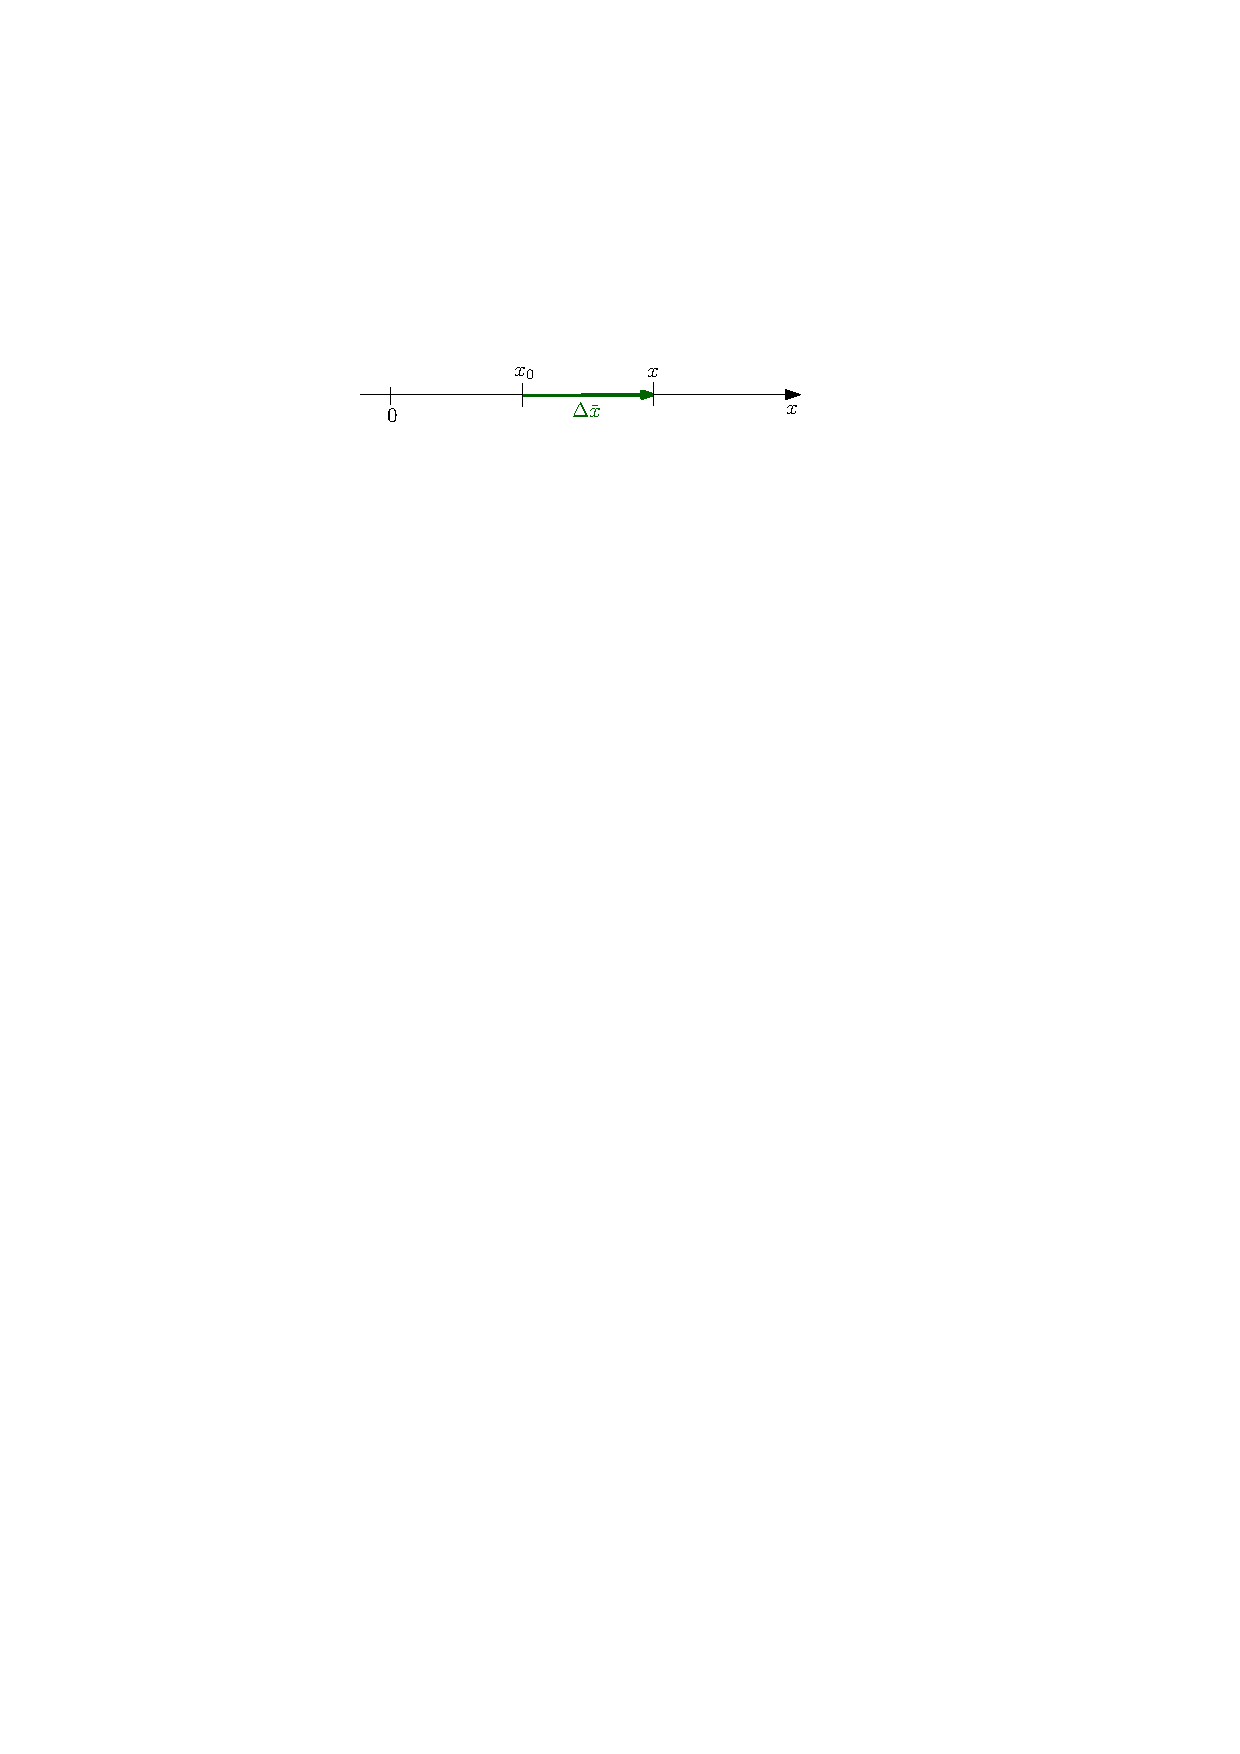
\includegraphics[width=.5\textwidth]{img/deltax.pdf}
  \caption{Desplazamiento en un movimiento rectilíneo.}
\end{figure}
en donde el {\bf módulo} del {\it vector desplazamiento} esta dado por: $$|\Delta \bar{x}| = \vert x - x_0 \vert$$

\info{En este curso, utilizaremos la letra griega $\mathbold{\Delta}$ (Delta mayúscula) para indicar {\bf \em variación}.
  Si, por ejemplo, nos encontramos con la expresión $\Delta a$, queremos decir ``el valor final de la magnitud $a$ menos su valor inicial $a_0$''. El subíndice cero siempre indicará el valor inicial de la magnitud que acompaña.}


Vamos a destacar que tanto el desplazamiento como la distancia recorrida se miden en {\bf metros (m)}, unidad base del SI y del SIMELA.
\bigskip


%%% % TABLA DE MAGNITUDES ESCALARES Y VECTORIALES

\begin{magnitud}{Magnitudes Físicas}
  En el curso anterior vimos que una magnitud quedaba definida en un proceso de medición. Teniendo en cuenta lo definido anteriormente, en este curso  necesitaremos distinguir entre dos tipos de magnitudes físicas:
  \begin{center}
  \begin{tabular}{|l|p{6cm}|p{6cm}|}
    \hline
    & Para definirlas se necesita        & Ejemplos\\
    \hline
    $\bullet$ Escalares:& $\rightarrow$ Un número real

                          $\rightarrow$ Una unidad de medida.
                          
                                         &
                                           \vspace*{-0.5\baselineskip}
                                           \begin{itemize}[leftmargin=*,nosep]
                                         \item[$\bullet$] 10\,\textordmasculine C
                                         \item[$\bullet$] 20 s
                                         \end{itemize}\\
                                           \hline
    $\bullet$ Vectoriales:& 
                            $\rightarrow$ Un vector, que consta de:
                            \begin{itemize}[nosep]
                            \item Una {\bf dirección} (recta sobre la que se encuentra)
                            \item Un {\bf sentido} (Indicado por una flecha)
                            \item Un {\bf módulo} (la medida del vector)
                            \end{itemize}
                            $\rightarrow$ Una unidad de medida.
                                         &
                                           \vspace*{-0.5\baselineskip}
                                           \begin{itemize}[leftmargin=*,nosep]
                                           \item[$\bullet$]  20 km/h en dirección Norte-Sur, hacia el Sur.
                                           \item[$\bullet$] 0,8 m en dirección vertical, hacia abajo.
                                           \end{itemize}
                                         \\
                                           
    \hline
  \end{tabular}
\end{center}
\end{magnitud}

\clearpage
\begin{comprension}
  {\bf Primero:}

Indica en los siguientes casos el desplazamiento {$\mathbold{\bar{d}}$} de una partícula que se mueve desde {$\mathbold{P_0}$} hasta {$\mathbold{P}$}:

\begin{figure}[H]
 \begin{subfigure}{0.5\textwidth}
    \centering
 	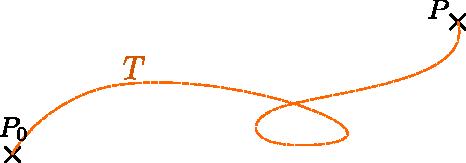
\includegraphics[width=.7\linewidth]{img/trayectoria_ej1.pdf}
	\caption{}	
\end{subfigure}   
 \begin{subfigure}{0.5\textwidth}
    \centering
 	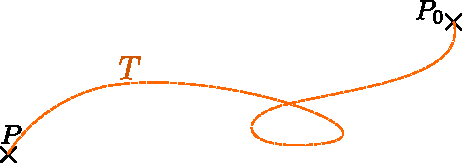
\includegraphics[width=.7\linewidth]{img/trayectoria_ej2.pdf}
	\caption{}	
\end{subfigure} 
 \begin{subfigure}{0.5\textwidth}
    \centering
 	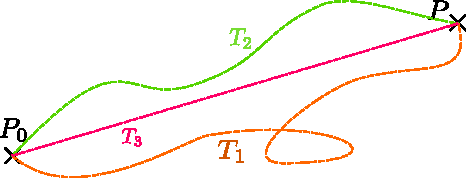
\includegraphics[width=.7\linewidth]{img/trayectoria_ej3.pdf}
	\caption{}	
\end{subfigure} 
 \begin{subfigure}{0.5\textwidth}
    \centering
 	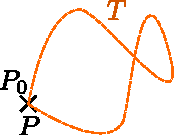
\includegraphics[width=.35\linewidth]{img/trayectoria_ej4.pdf}
	\caption{}	
\end{subfigure}
\end{figure}

\noindent
{\bf Segundo:}

Indica en los siguientes casos la {\it trayectoria}, el {\it desplazamiento } ($\mathbold{\Delta \bar{x}}$) y la {\it distancia recorrida}:

\begin{figure}[H]
 \begin{subfigure}{0.5\textwidth}
    \centering
 	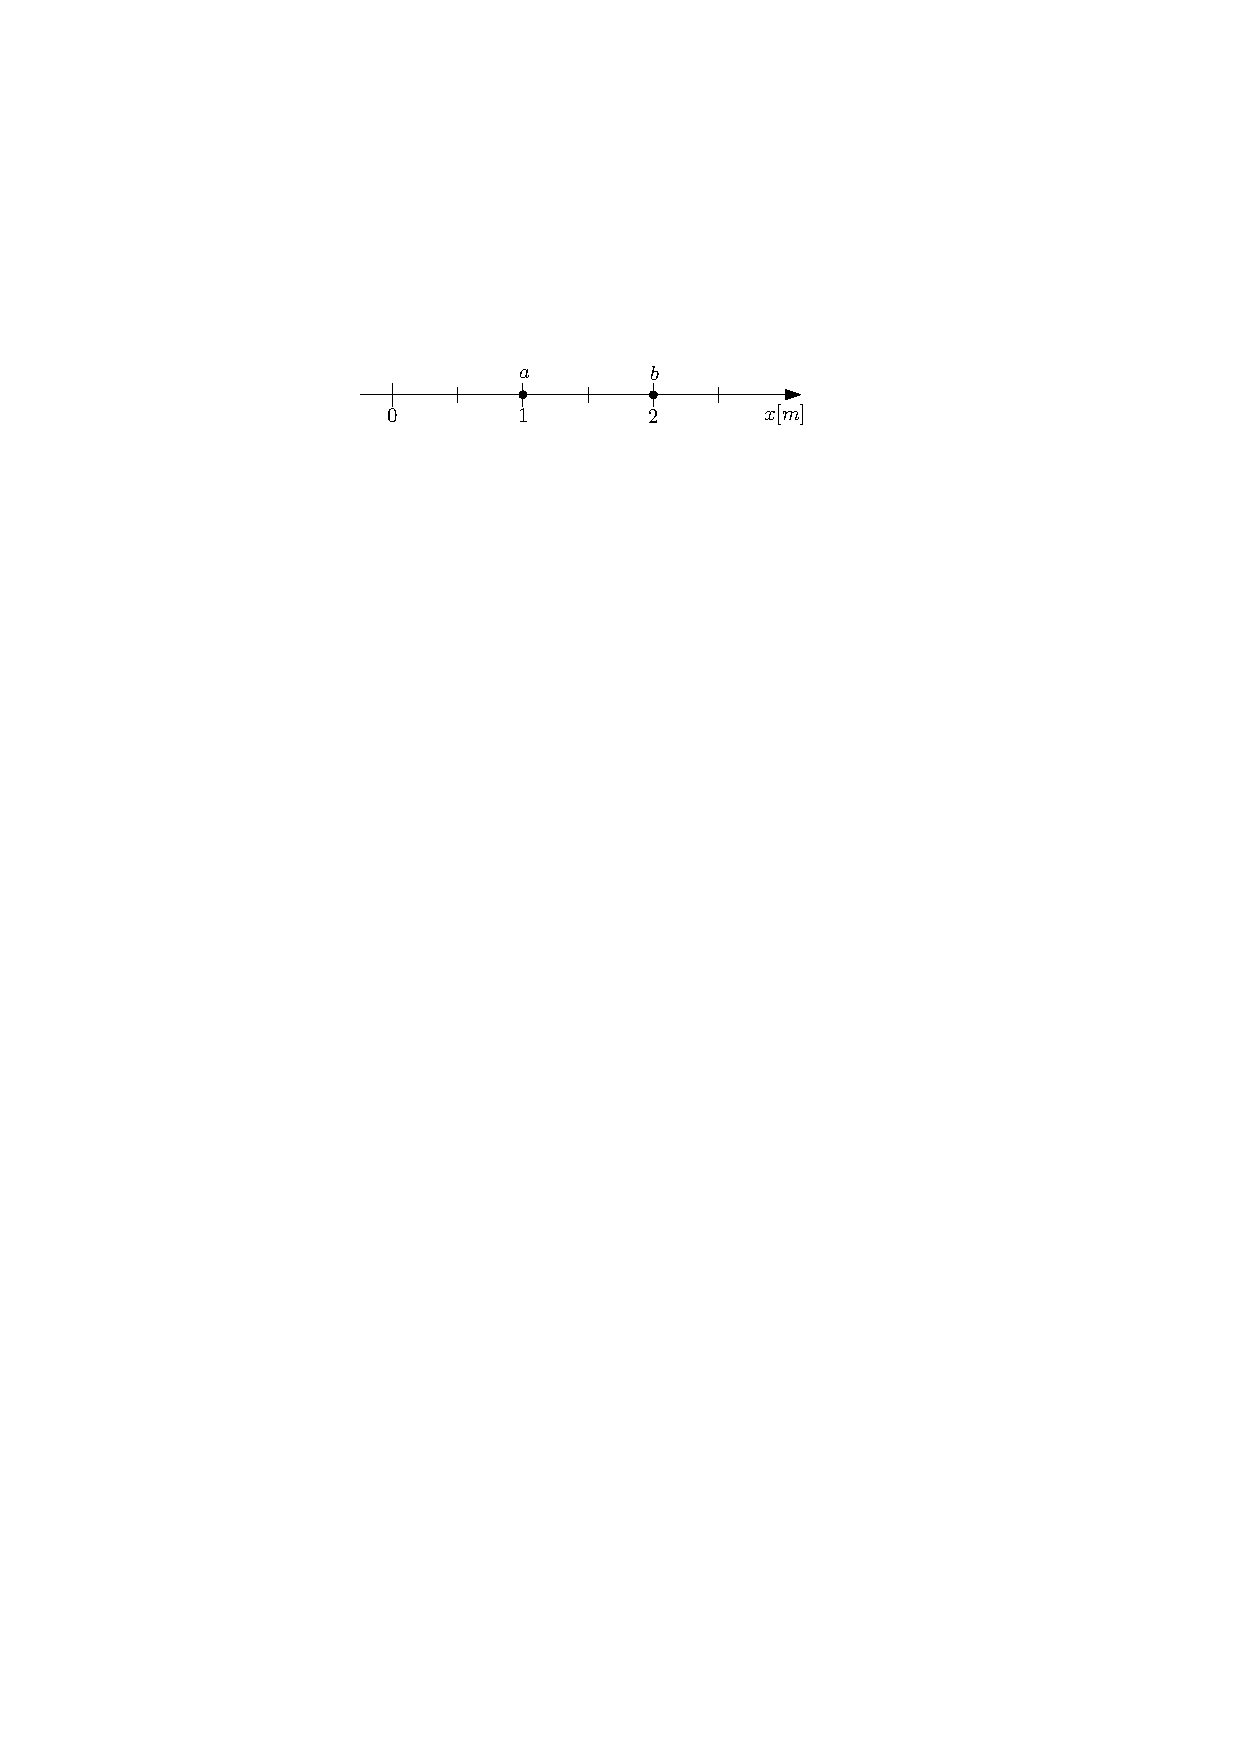
\includegraphics[width=.9\linewidth]{img/p_t_d_ej1.pdf}
	\caption{Una partícula se mueve desde $a$ hasta $b$.}	
\end{subfigure}   
 \begin{subfigure}{0.5\textwidth}
    \centering
 	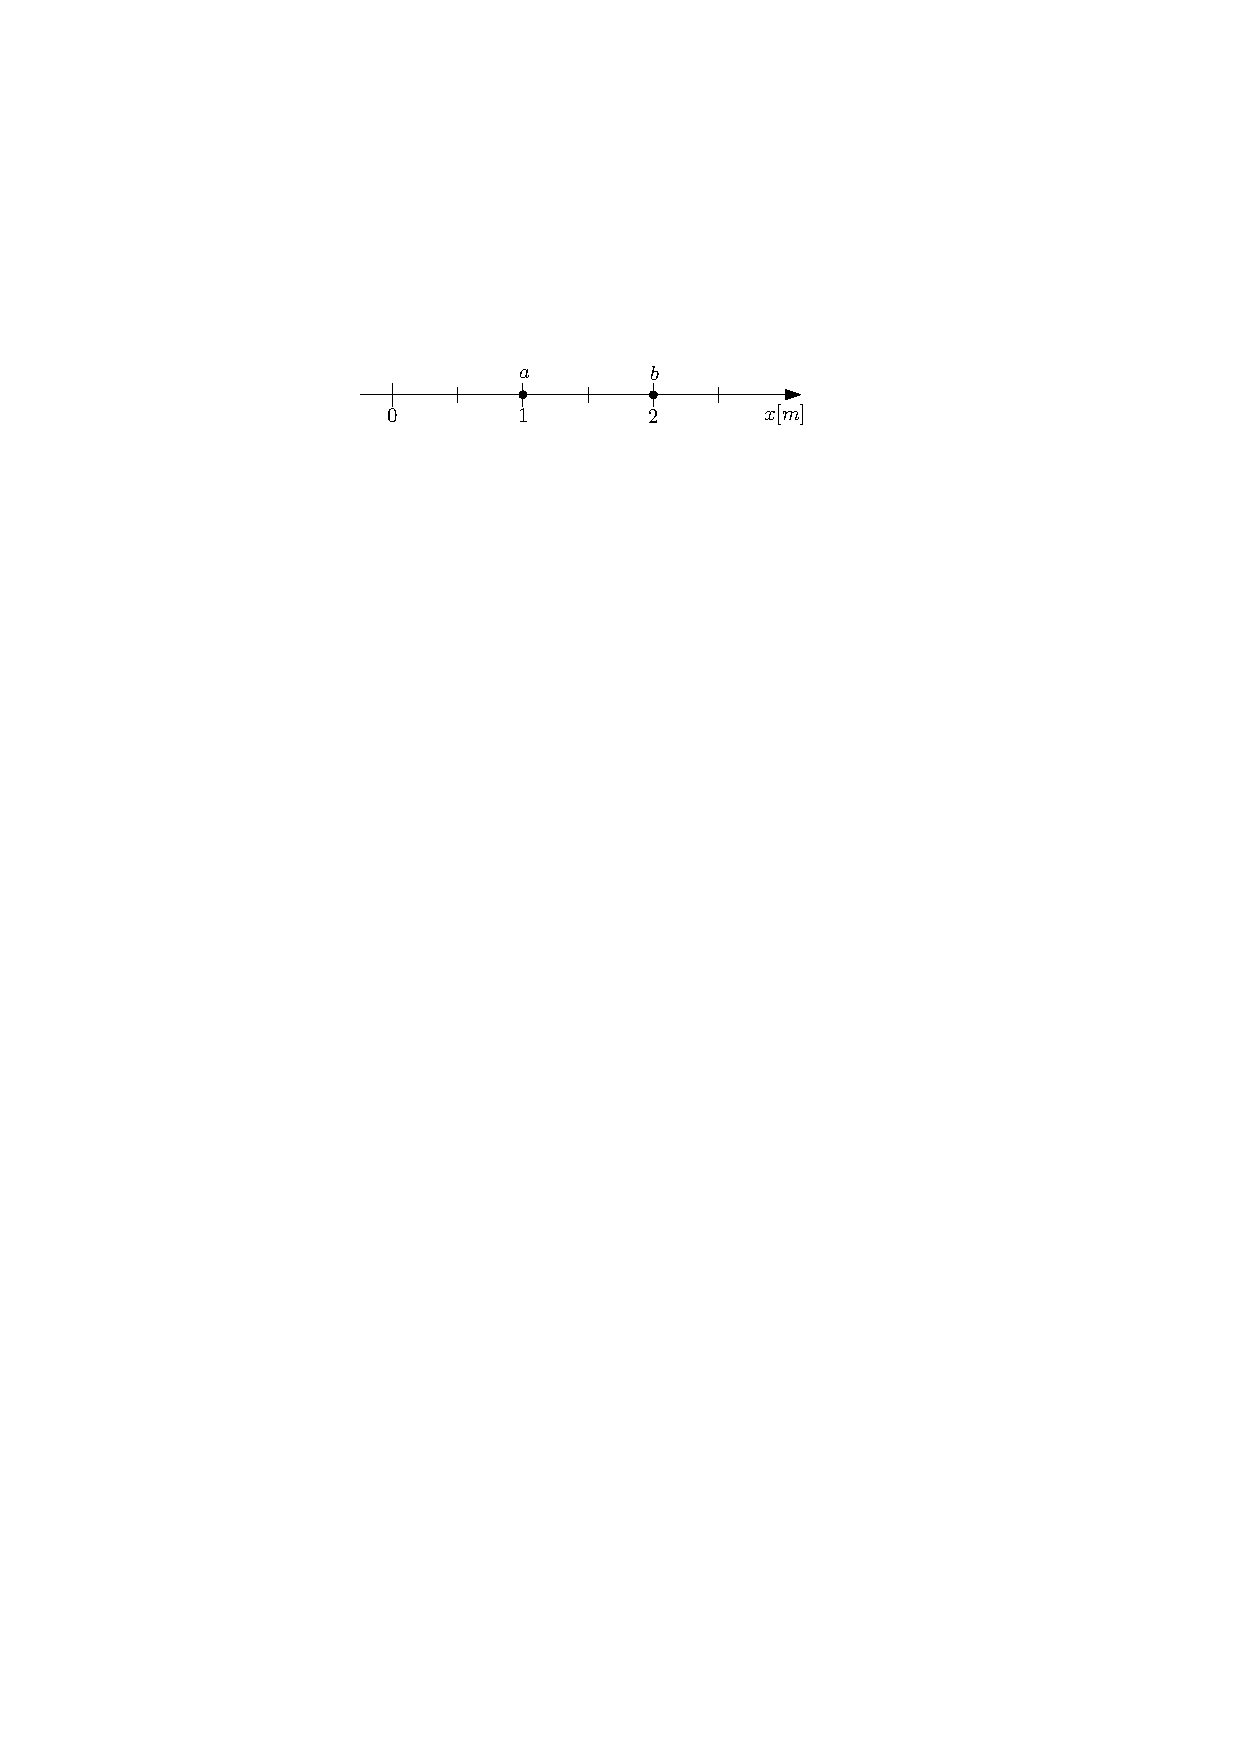
\includegraphics[width=.9\linewidth]{img/p_t_d_ej1.pdf}
	\caption{Una partícula se mueve desde $b$ hasta $a$.}	
\end{subfigure}
 \begin{subfigure}{0.5\textwidth}
    \centering
 	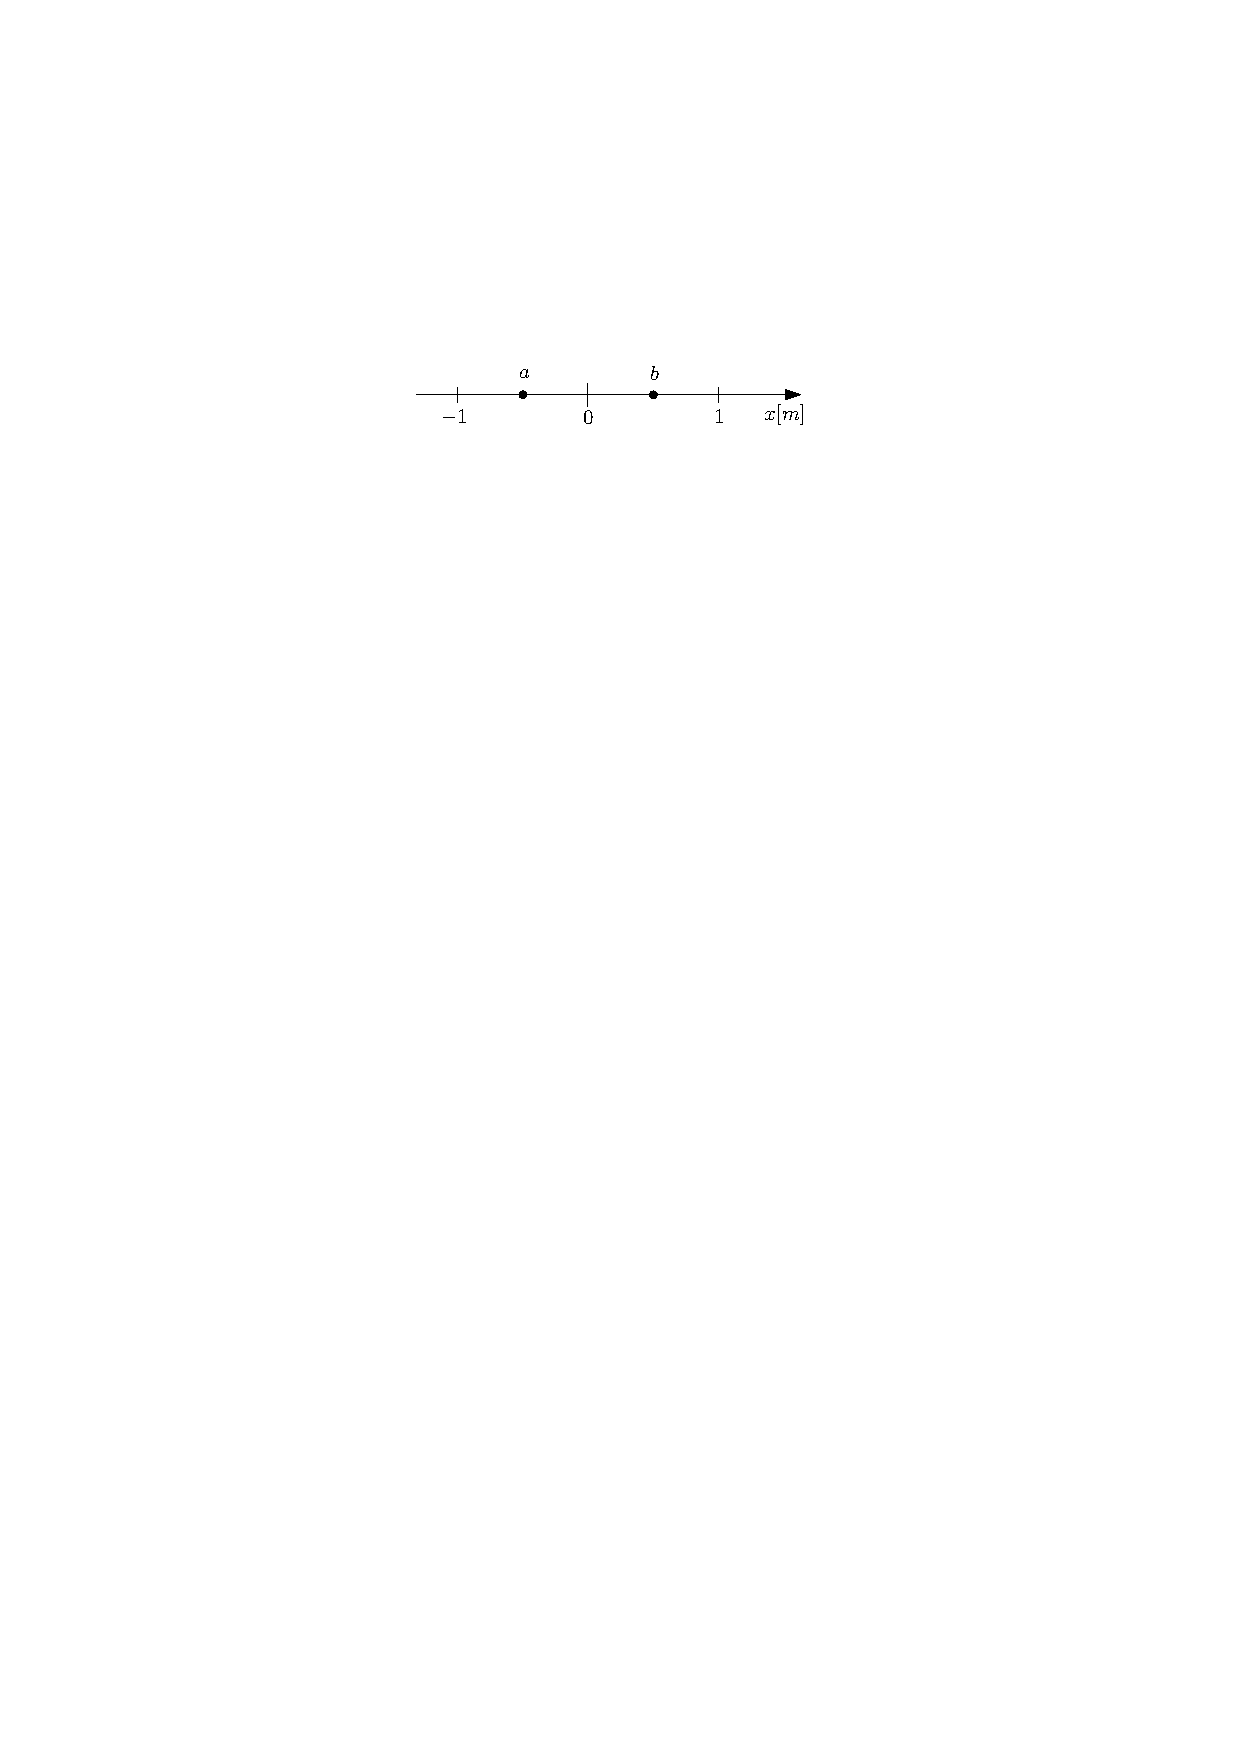
\includegraphics[width=.9\linewidth]{img/p_t_d_ej3.pdf}
	\caption{Una partícula se mueve desde $a$ hasta $b$ y luego de $b$ hacia $a$}	
\end{subfigure} 
 \begin{subfigure}{0.5\textwidth}
    \centering
 	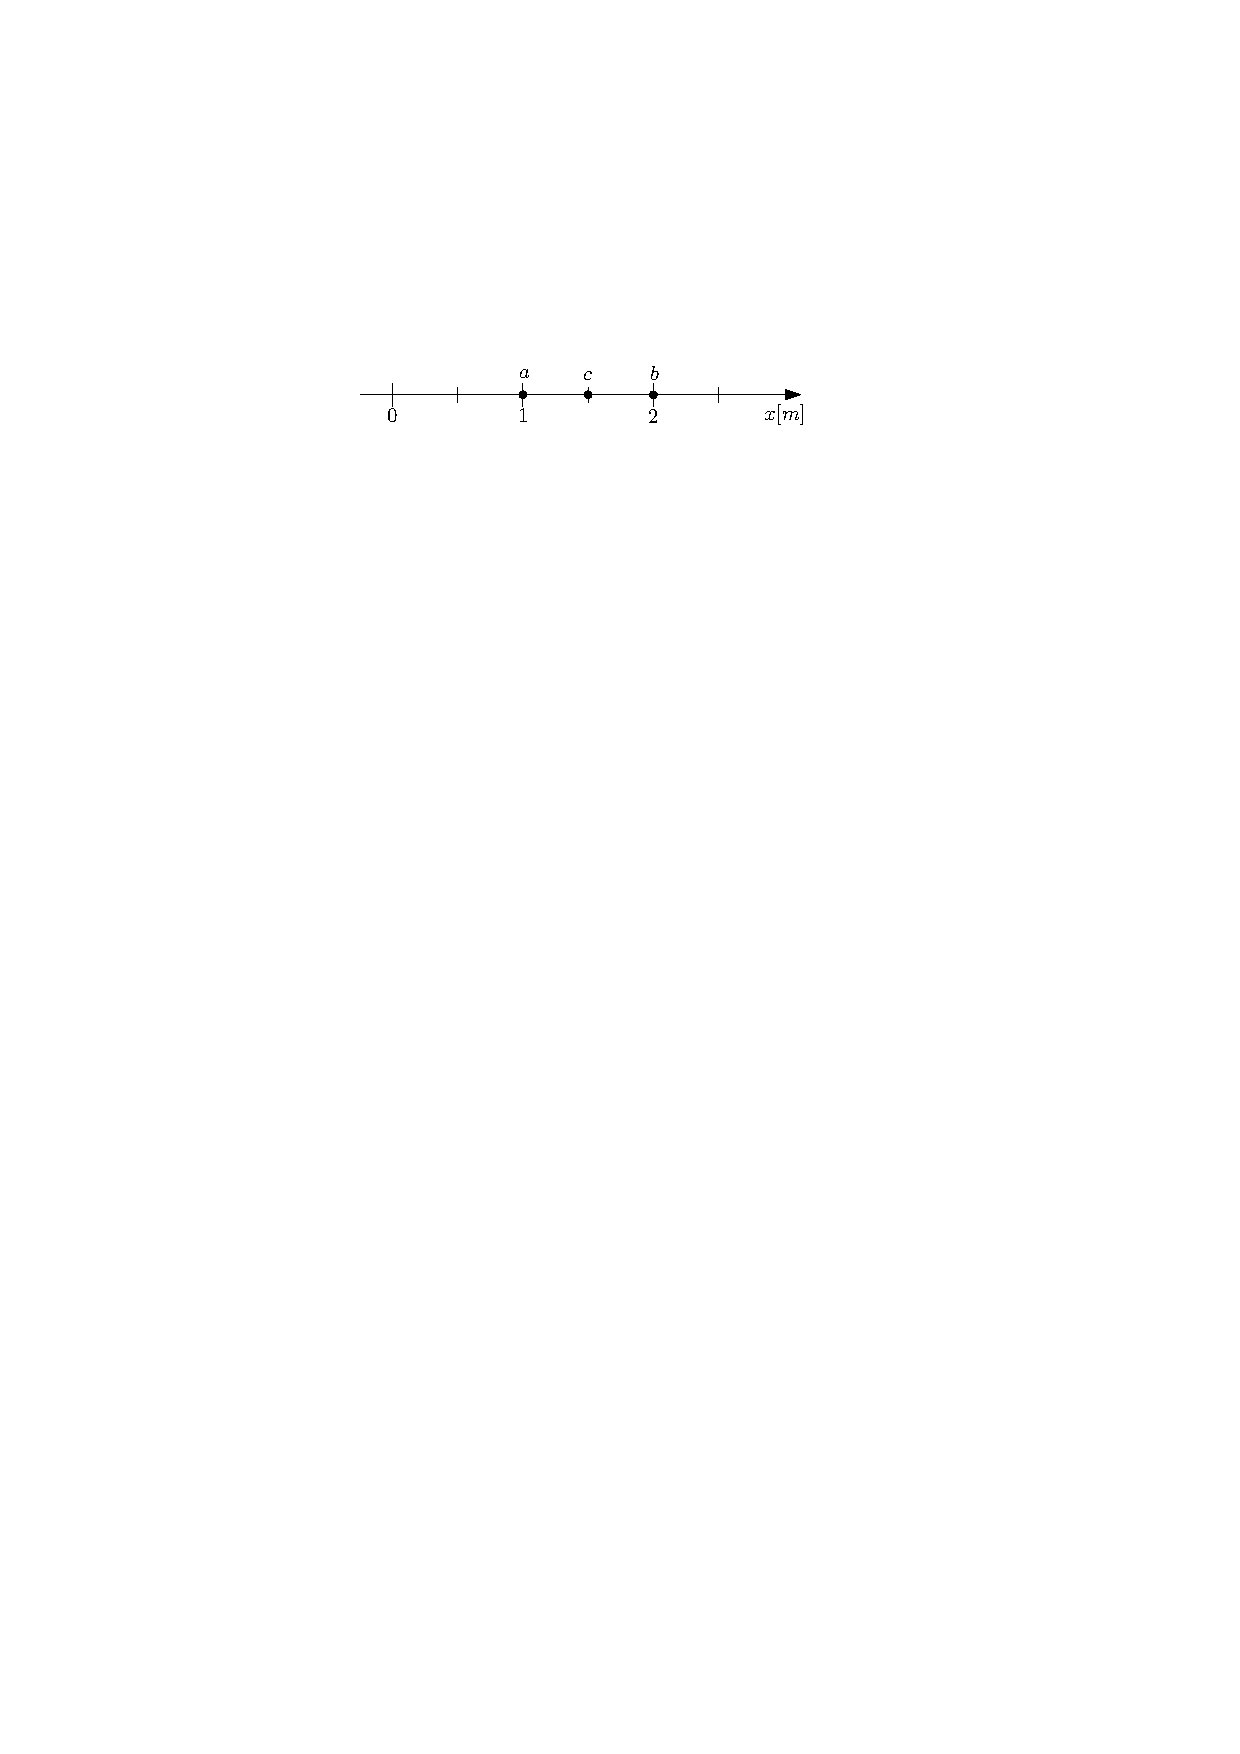
\includegraphics[width=.9\linewidth]{img/p_t_d_ej2.pdf}
	\caption{Una partícula se mueve desde $a$ hasta $b$ y finalmente hasta $c$.}	
\end{subfigure} 
\end{figure}

\noindent
{\bf Tercero:}

En base a lo que has pensado anteriormente, responde:
\begin{enumerate}
\item ¿Puede una partícula recorrer una distancia y que su desplazamiento sea nulo?
\item En una trayectoria rectilínea, ¿coincide siempre la distancia recorrida con el módulo del desplazamiento?
\end{enumerate}
\end{comprension}

\section{Velocidad}

\subsection{Velocidad media}

La \textbf{velocidad media }de una partícula se define como la razón entre su desplazamiento {$\mathbold{\bar{d}}$} y el intervalo de tiempo $\Delta t$ en que se produce dicho desplazamiento:

$$\mathbold{\bar{v}_m}\ = \ \frac{\mathbold{\bar{d}}}{\Delta t}$$

en donde dicha velocidad es una magnitud {\it vectorial} la cual tiene la misma dirección y sentido que el desplazamiento debido a que $\Delta t > 0$.


En el caso particular de un movimiento rectilíneo, la velocidad media queda de la forma:

\begin{center}
\boxed{\mathbold{\bar{v}_m} \ = \ \frac{\mathbold{\Delta \bar{x}}}{\Delta t}}
\end{center}

gráficamente:

\begin{figure}[h!]
\center
 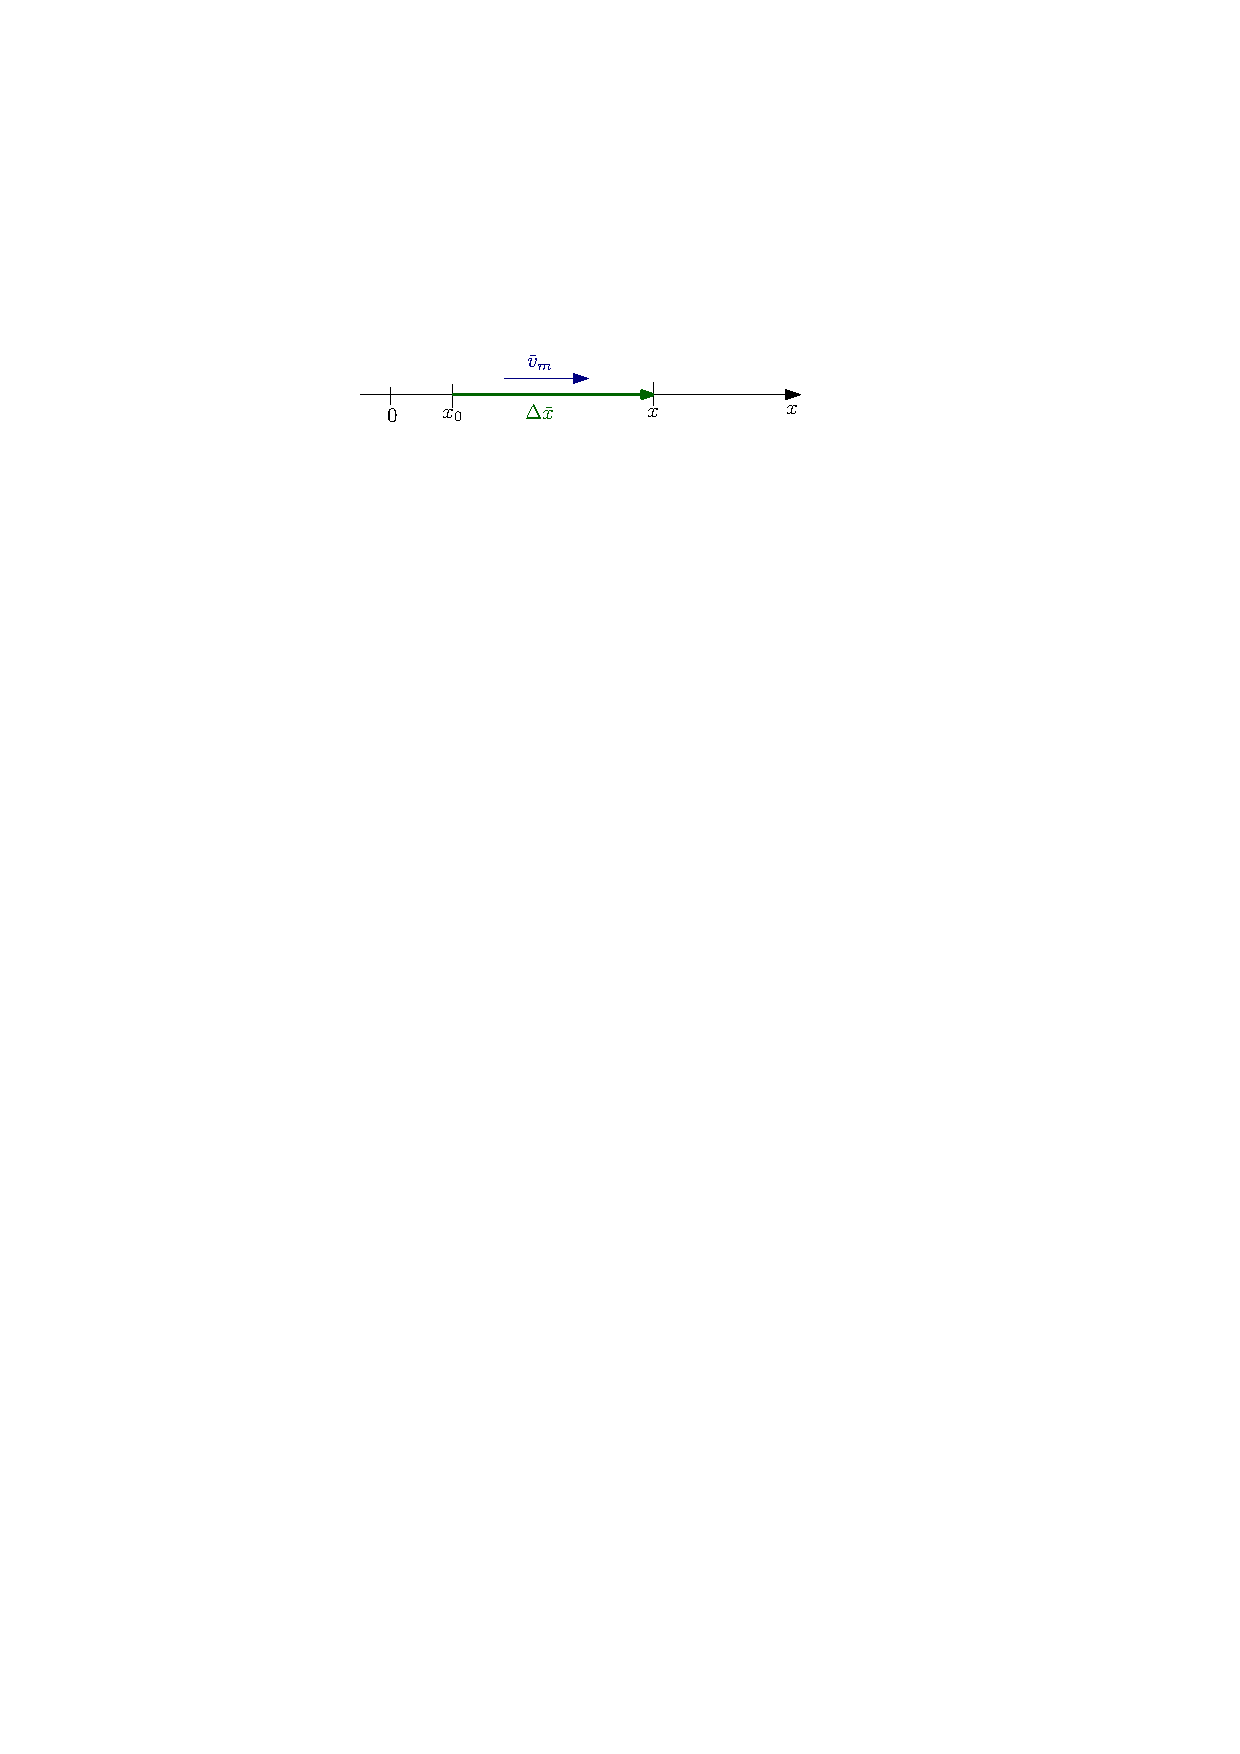
\includegraphics[width=.5\textwidth]{img/vm.pdf}
  \caption{Velocidad media en un movimiento rectilíneo.}
\end{figure}


Las unidades con que se miden las velocidades surgen de la misma operación que las define. Se trata de un cociente entre una longitud ($\Delta x$) y un intervalo de tiempo ($\Delta t$). Con esta expresión: $$[v_m] = \frac{[\Delta x]}{[\Delta t]}$$
Si trabajamos en el SIMELA, la unidad derivada es:$$[v_m] = \sif{m}{s}$$

\begin{comprension}

  \noindent{\bf Primero:}

Supongamos que un automóvil está viajando hacia Rosario. ¿Que le preguntarías al conductor para determinar la \textit{velocidad media} de su movimiento?

\noindent
{\bf Segundo:}

Un automóvil se desplaza desde Rosario hasta Buenos Aires como muestra la figura. Dicho móvil tarda 3 horas en llegar a destino. Determina la velocidad media del automóvil entre las ciudades de Rosario y Buenos Aires.


\begin{figure}[H]
\centering
 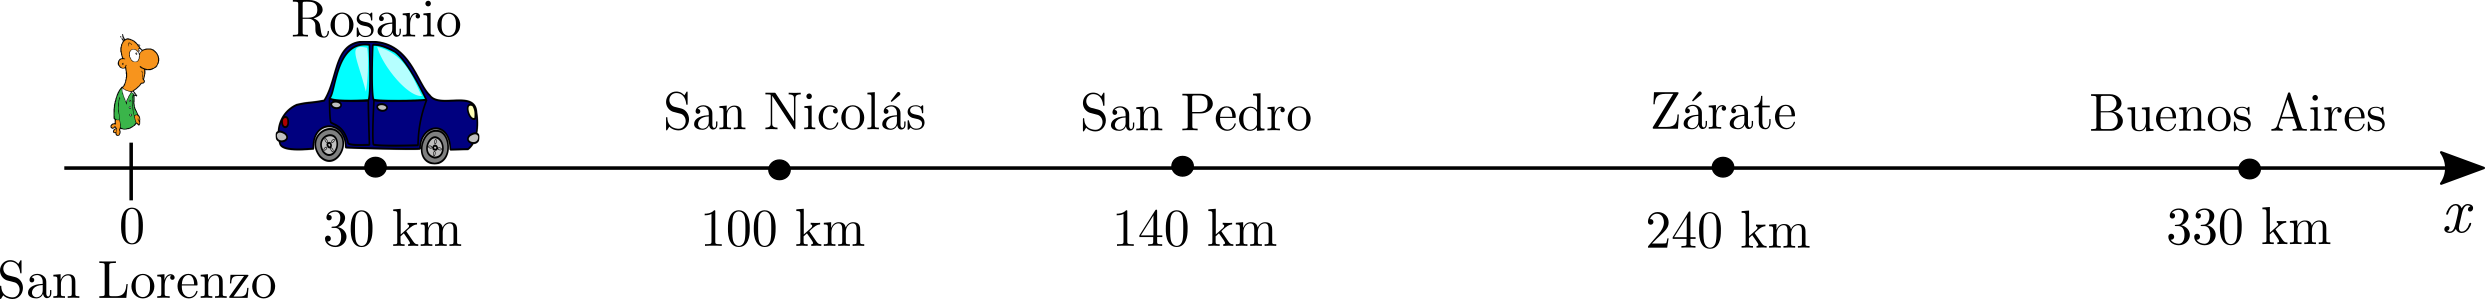
\includegraphics[width=.9\textwidth]{img/viaje.png}
 % \caption{Velocidad media en un movimiento rectilíneo.}
\end{figure}

Para ayudarte, representa gráficamente las posiciones inicial y final, el desplazamiento y luego la velocidad media:

\begin{figure}[H]
\centering
 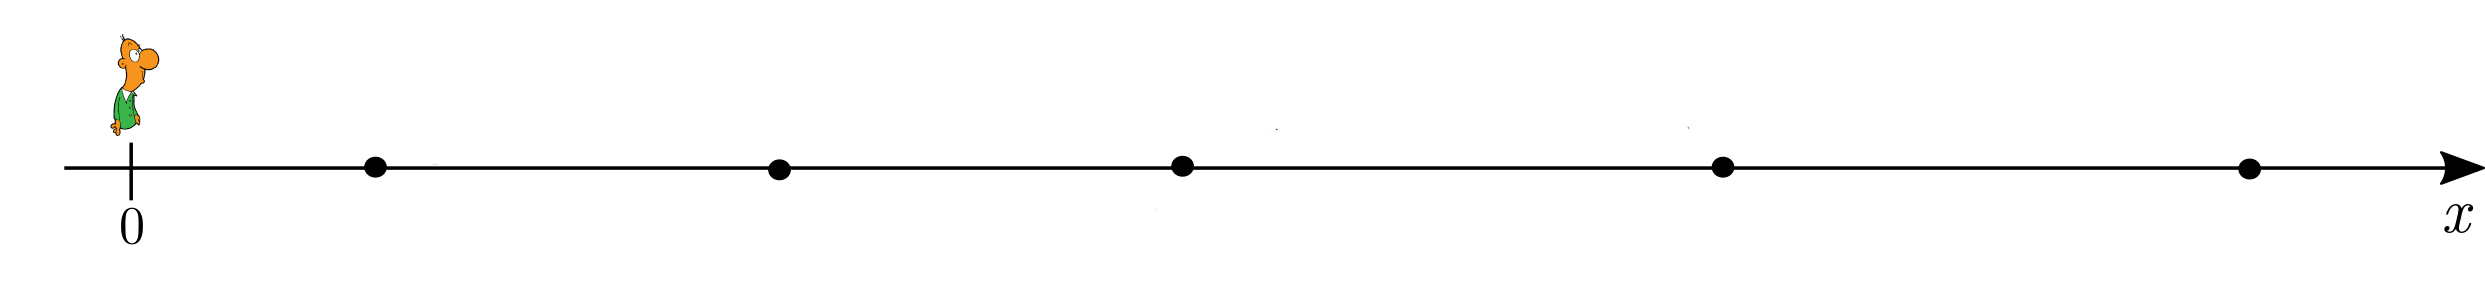
\includegraphics[width=.9\textwidth]{img/viaje2.png}
 % \caption{Velocidad media en un movimiento rectilíneo.}
\end{figure}



A partir de la información de la velocidad media conseguida. ¿Podemos saber cuál era la velocidad del automóvil cuando pasaba por San Nicolás? ¿Y por Zárate? ¿Podemos saber si se detuvo a descansar en San Pedro?
\end{comprension}

\subsection{Velocidad Instantánea}

\info{
    Antes de definir {\it velocidad instantánea} debemos destacar que la palabra {\bf instante} tiene un significado un poco distinto en física que en el lenguaje cotidiano. Podemos utilizar la frase ``duró sólo un instante'' para referirnos a algo que duró un intervalo de tiempo muy corto. Sin embargo, en física un instante no tiene duración; es un solo valor de tiempo.}

Podemos definir la {\bf velocidad instantánea} como la velocidad de una partícula en cualquier {\it instante} de tiempo.

Supongamos que una partícula viaja desde {$\mathbold{P_0}$} hasta {$\mathbold{P}$} por la trayectoria {$\mathbold{T}$}, definiendo un desplazamiento {$\mathbold{\bar{d}}$}:

La velocidad media de este movimiento podríamos determinarla: $\mathbold{\bar{v}_m}=\frac{\mathbold{\bar{d}}}{\Delta t}$

\begin{figure}[!h]
\centering
 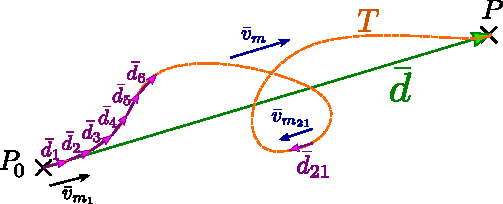
\includegraphics[width=.6\textwidth]{img/velocidad_instantanea.pdf}
 \caption{\label{fig:particion_tray} Una trayectoria cualquiera se puede dividir en pequeños intervalos. En cada intervalo, el desplazamiento se parecerá mucho más a la trayectoria.}
\end{figure}


Si dividimos la trayectoria total en pequeñas trayectorias, como muestra la Figura~\ref{fig:particion_tray}, podríamos definir pequeños intervalos de desplazamiento ({$\mathbold{\bar{d}_1; \bar{d}_2;...}$}). Observemos que cada uno de estos desplazamientos ocurren en ciertos intervalos de tiempo ({$\Delta t_1; \Delta t_2;...$}). Así, podremos calcular también distintas velocidades medias para cada uno de estos intervalos. 

Tomemos, como ejemplo, que el desplazamiento {$\mathbold{\bar{d}_{21}}$} ocurre en el intervalo de tiempo {$\Delta t_{21}$} por lo tanto, la partícula, en ese intervalo, tendría una velocidad media dada por: $$\mathbold{\bar{v}_{m_{21}}} = \frac{\mathbold{\bar{d}_{21}}}{\Delta t_{21}}$$

Vemos que la velocidad $\mathbold{\bar{v}_{m_{21}}}$ describe mucho mejor el comportamiento de la partícula en ese tramo de trayectoria que la velocidad $\mathbold{\bar{v}_m}$.

Si tomamos intervalos de tiempo cada vez más chicos, veremos que los valores de velocidad media se acercan a los de velocidad instantánea. ¡Y así podremos saber cuál es la velocidad del automóvil en el instante en que pasa por San Pedro!

Podemos decir que a medida que el intervalo de tiempo {\em tiende a cero} o se aproxima lo suficientemente a cero,  la velocidad media tiende a la velocidad instantánea, en cada intervalo considerado. El concepto matemático de aproximación a un valor pero sin llegar al mismo se denomina {\bf \em límite}. La definición rigurosa de {\bf \em velocidad instantánea} usa dicho concepto:
$$\mathbold{\bar{v}_{m_{21}}} = \lim_{\Delta t \rightarrow 0} \mathbold{\bar{v}_m} = \lim_{\Delta t \rightarrow 0}\frac{\mathbold{\bar{d}}}{\Delta t}$$
Sin embargo, en nuestro caso, lo importante no es usar esta definición matemáticamente rigurosa, sino comprender conceptualmente lo que acabamos de analizar.

En el caso particular de un movimiento rectilíneo, la velocidad instantánea queda de la forma:
$$\mathbold{\bar{v}} = \lim_{\Delta t \rightarrow 0} \mathbold{\bar{v}_m} = \lim_{\Delta t \rightarrow 0} \frac{\mathbold{\Delta \bar{x}}}{\Delta t}$$


La velocidad es una magnitud vectorial. Pensemos en dos automóviles que se mueven por la misma ruta en sentidos opuestos a 60 km/h y 70 km/h respectivamente. Refiriendo estas velocidades al sistema de coordenadas resultarán de signos opuestos:

%% Acá hay que ponerse de acuerdo en cómo vamos a decir lo del signo.

\begin{figure}[h!]
\centering
 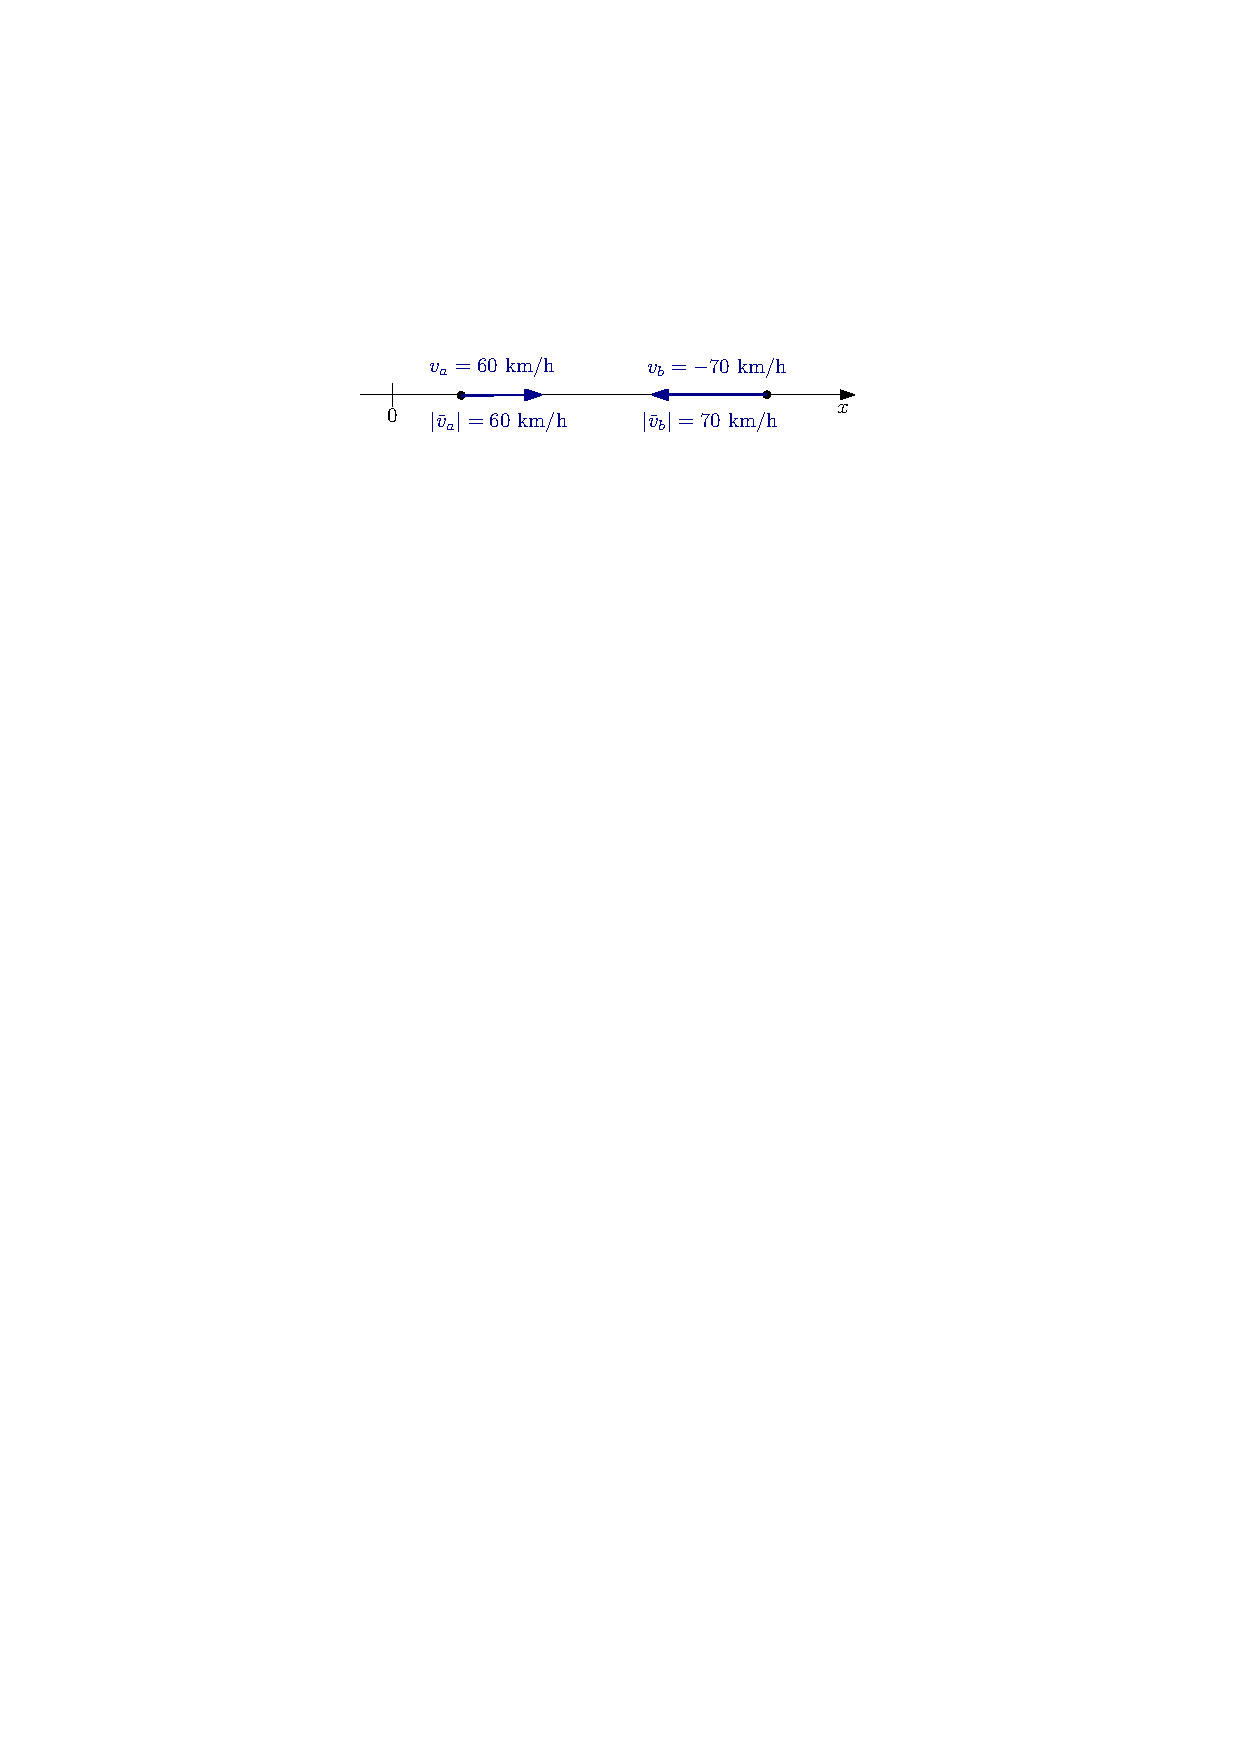
\includegraphics[width=.6\textwidth]{img/velocidad_instantanea2.pdf}
 % \caption{Velocidad media en un movimiento rectilíneo.}
\end{figure}
El signo de la velocidad \textbf{depende del sistema de coordenadas} y nos indica el sentido del movimiento.


{\bf \color{BrickRed} {¡Cuidado!}} En el ejemplo anterior, cuando decimos ``$v_a= 60$ km/h'' o ``$v_b= -70$ km/h'', {\bf ¡nos estamos refiriendo a la componente $\mathbold{x}$ del vector velocidad!} Debido a que el movimiento es rectilíneo, es decir que la partícula se mueve en el eje $x$, podemos utilizar esta notación. Si el movimiento fuera en un plano deberíamos escribir sus dos componentes:

\begin{figure}[h!]
\centering
 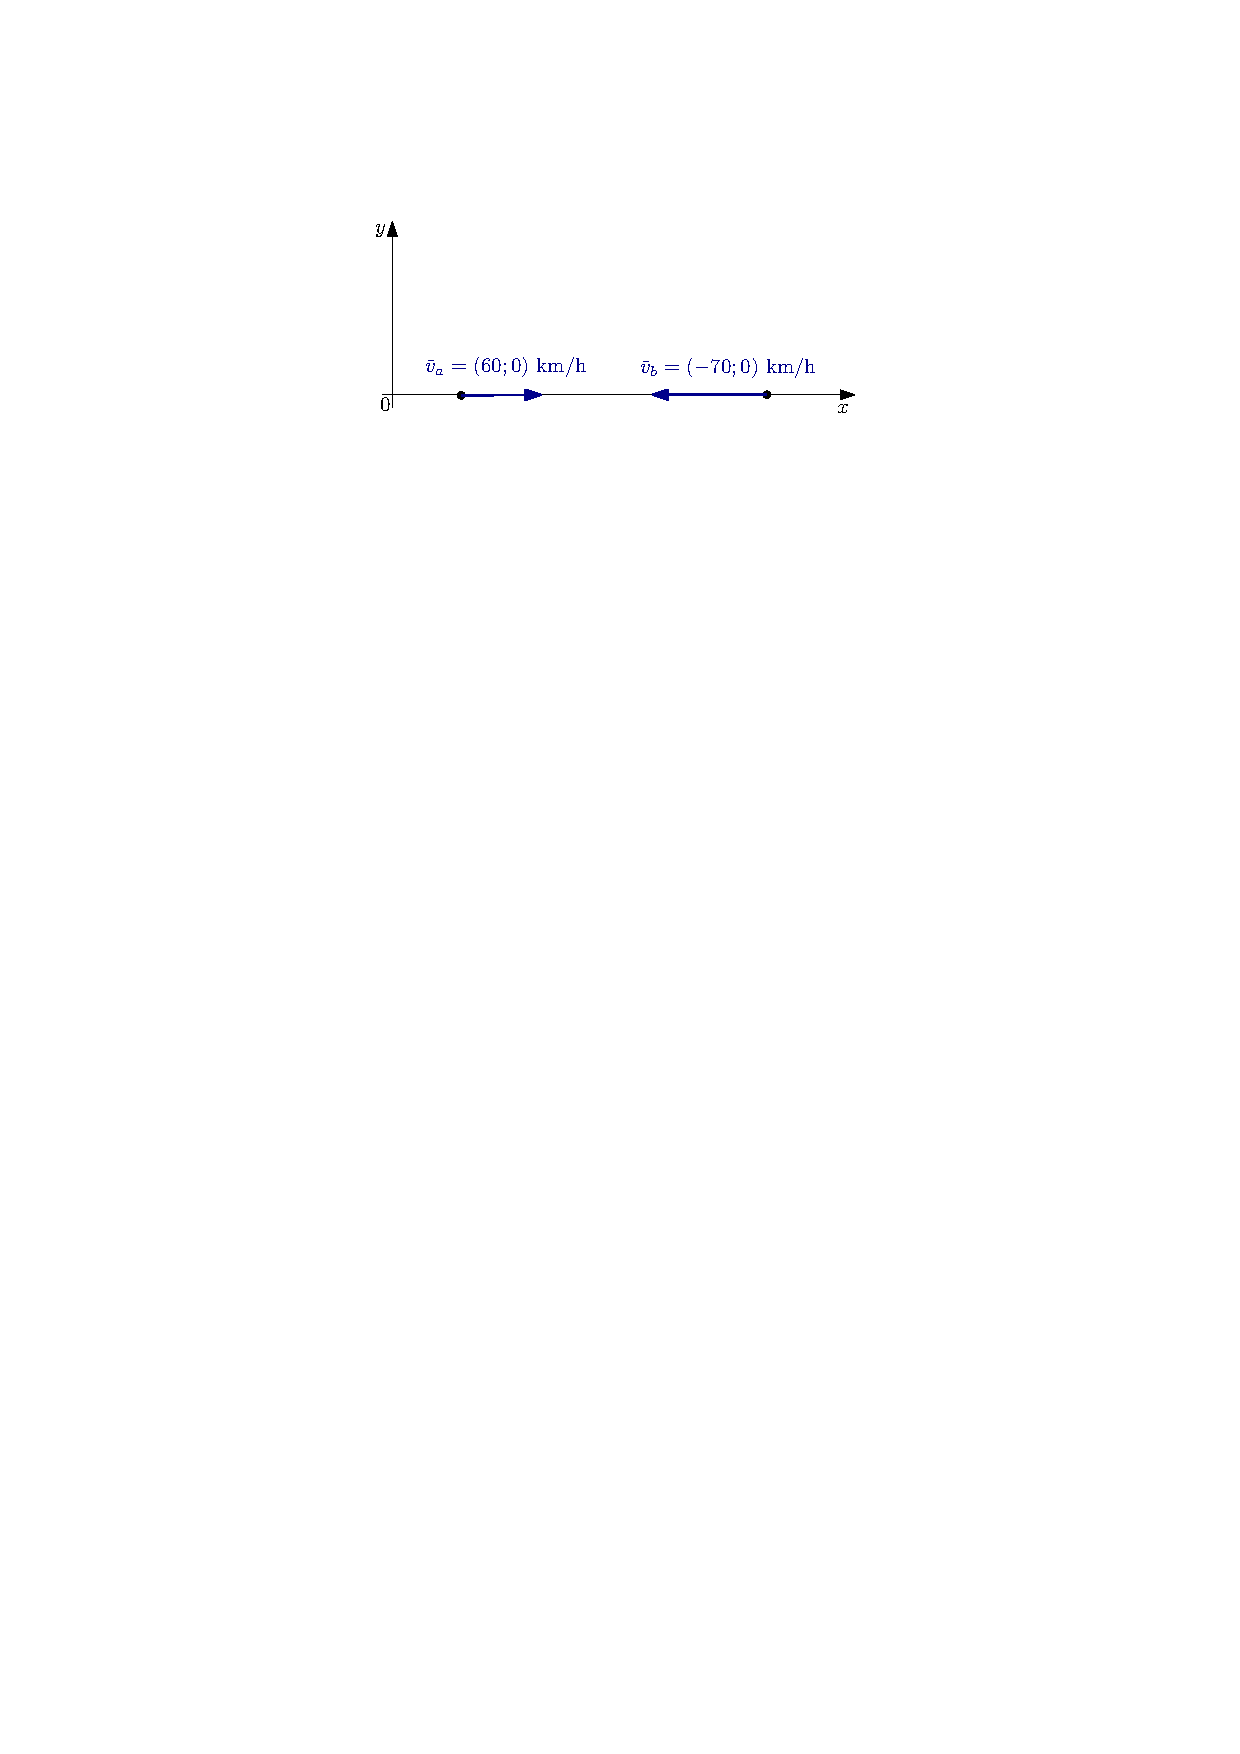
\includegraphics[width=.6\textwidth]{img/velocidad_instantanea3.pdf}
 % \caption{Velocidad media en un movimiento rectilíneo.}
\end{figure}

La \textbf{rapidez} de una partícula se define como el {\bf ``módulo''} de su velocidad. La rapidez no tiene dirección asociada y, en consecuencia, no lleva signo algebraico. Por ejemplo si una partícula tiene una velocidad de +25 m/s y otra de –25 m/s sobre el eje $x$, las dos tienen una rapidez de 25 m/s. El velocímetro de un automóvil indica la rapidez instantánea y no la velocidad instantánea.



%%%%%%%%%%%%%%%%%%
% \end{document}
 